\documentclass[a4paper,12pt]{article}
\usepackage[polish]{babel}
\usepackage{polski}
\usepackage[utf8]{inputenc}
\usepackage[T1]{fontenc}
\usepackage[margin=1.5cm]{geometry}
\usepackage{longtable}
\usepackage{graphicx}
\usepackage{float}
\usepackage{pdfpages}


\title{Wizualizacja danych sonaru}
\author{Dorian Janiak}
\date{14.05.2015}

\begin{document}

\maketitle

\section{Krótki opis}
Projekt zakłada stworzenie aplikacji komputerowej, która będzie wizualizowała
otrzymywane dane z sonaru ultradźwiękowego. Aplikacja ma próbować łączyć dane
w taki sposób, aby móc z nich stworzyć zarys otoczenia. Drugą część projektu
stanowi symulacja, której zadaniem jest z odpowiednio przygotowanych obiektów
geometrycznych wygenerować dane potrzebne do wykonania wizualizacji 
(ma być symulacją sonaru). 
Dane mają zostać przesłane przy pomocy wybranego protokołu komunikacyjnego.

\section{Cel}
Celem projektu jest zapoznanie się ze środowiskiem Qt oraz sposobami wizualizacji danych.
Jednym z problemów, który zostanie również poruszony w ramach pracy będzie 
sposób komunikacji modułów i przesył danych. Jednym z ważnych powodów podjęcia się realizacji tego tematu
jest chęć głębszego poznania biblioteki OpenGL. 

\section{Rozszerzony opis}
\subsection{Komputer PC}
Projekt składa się z dwóch części. Pierwsza część obejmuje stworzenie aplikacji
w Qt, która pozwoli na przedstawienie danych sensorycznych z sonaru.
Sonar i robot mobilny zostaną stworzone w ramach osobnego projektu (kurs: Roboty mobilne(1)).
Aplikacja stworzona w środowisku Qt pozwala również na sterowanie robotem. 
Dane są wysyłane do robota przy użyciu interfejsu Bluetooth. Robot reaguje na to zmieniając swoją
pozycję. Następnie z aplikacji Qt wysyła się żądanie wykonania skanowania terenu. 
Robot przy pomocy czujnika ultradźwiękowego rozpoczyna skanowanie terenu, zapisując dane w
swojej pamięci. Gdy skończy - przesyła dane pomiarowe przez interfejs Bluetooth do komputera z 
aplikacją. Dane zostają wczytane i zwizualizowane. Należy przy tym pamiętać, że robot
nie znajduje się dokładnie w tym miejscu, w którym oczekiwalibyśmy. Dane zostają połączone
przez aplikację i wyrysowany zostaje kolejny kawałek mapy otoczenia. Gdyby omiatanie terenu
odbywało się również wertykalnie, a nie tylko horyzontalnie możnaby wymagać większej
dokładności wizualizacji.
\subsection{Urządzenie} 
Drugą częśc aplikacji stanowi symulator robota z sonarem. Początkowym założeniem było stworzenie symulatora uruchamianego
na tym samym komputerze co główna aplikacja, jednak po rozpoznaniu tematu i ponownym oszacowaniu dostępnego czasu projekt symulatora
został ograniczony do projektu aplikacji na urządzenie z systemem Android.
Aplikacja będzie wczytywać obiekty z plików OBJ oraz ze specjalnych plików konfiguracyjnych
położenie poszczególnych obiektów na scenie (proponowany format: JSON). Następnie będzie
omiatała otoczenie z pewną dokładnością. Wyniki zostaną wysłane poprzez interfejs Bluetooth. Posłużą one
do zwizualizowania efektów symulacji w oknie aplikacji z pierwszej części. 
Ostatnim etapem rozwoju symulatora będzie stworzenie ciągłej komunikacji między symulatorem i aplikacją
wizualizującą, tak aby można było sterować robotem umieszczonym w symulatorze.


\section{Funkcjonalność skończona}
Poniżej zamieszczona została lista funkcjonalności, którą udało się ukończyć dotychczas. Lista zawiera również nieplanowany wcześniej punkt. 
Został on zrealizowany w celu ułatwienia późniejszego debugowania i wyszukiwania problemów w trakcie komunikacji z urządzeniem. Klasa (MessageController)
została specjalnie stworzona w taki sposób, aby dziedzicząc ją była w stanie obsłużyć zarówno dane pochodzące z pliku dyskowego jak i dane pochodzące z 
transmisji Bluetooth. 
\textit{W nawiasach zostały zamieszczone dodatkowe uwagi odnośnie punktowanych funkcjonalności} 
\subsection{Aplikacja na komputerze PC}
\begin{itemize}
\item Rysowanie na scenie 3D mapy otoczenia.
\item Wczytywanie danych pomiarowych sonaru z pliku (w przypadku symulacji).
\item Łączenie nowo odczytanej z poprzednio odczytaną mapą terenu. 
\item Możliwość sterowania widokiem 3D.
\item \textit{ (Nieplanowane wcześniej) }Wyświetlanie logów dotyczących przesyłanych komunikatów oraz interpretacja występujących błędów.
\item \textit{ (Zrealizowane w okresie między 1. i 2. raportem) } Rysowanie na scenie 3D robota.
\item \textit{ (Zrealizowane w okresie między 1. i 2. raportem) } Udostępnienie pilota pozwalającego na sterowanie robotem (lub symulacją).
\end{itemize}

\subsection{Symulator na urządzeniu}
\begin{itemize}
\item \textit{ (Zrealizowane w okresie między 1. i 2. raportem) } Ładowanie plików OBJ, parsowanie oraz logowanie wczytanych informacji
\end{itemize}


\section{Funkcjonalność planowana}
Poniżej zamieszczone zostały listy funkcjonalności, które zamierzam wykonać w ramach projektu. 
\subsection{Aplikacja na komputerze PC}
\begin{itemize}
\item Wysyłanie żądania przemieszczenia robota (poprzez interfejs komunikacyjny).
\item Wysyłanie żądania wykonania skanowania terenu (poprzez interfejs komunikacyjny).
\item Odbieranie danych z sonaru robota (poprzez interfejs komunikacyjny).
\end{itemize}

\subsection{Symulator na urządzeniu}
\begin{itemize}
\item Prosta symulacja sonaru ultradźwiękowego
\item Wysłanie danych do aplikacji wizualizującej poprzez interfejs komunikacyjny (Bluetooth)
\item Odbieranie żądania przemieszczenia robota na scenie
\item Odbieranie żądania wykonania symulacji i przesłania wyników
\end{itemize}

\section{Funkcjonalność zawieszona}
Funkcjonalność wymieniona w tym punkcie została zawieszona ze względu na ograniczenia czasowe oraz stosunkowo małą jej przydatność w programie.
Symulator stworzony na komputerze PC przy poniższych założeniach nie jest w stanie dorównać symulatorowi zainsalowanemu na urządzeniu zewnętrznym, z którym
program będzie musiał komunikować się poprzez interfejs Bluetooth. Czas, który pierwotnie miał być poświęcony na jej stworzenie zostanie przeznaczony
na stworzenie symulatora na telefonie z systemem Android.
\subsection{Symulator na komputerze PC}
\begin{itemize}
\item Ładowanie plików konfiguracyjnych (zawierają informacje o położeniu obiektów 3D na symulowanej scenie)
\item Ładowanie plików OBJ
\item Symulacja sonaru ultradźwiękowego
\item Zapisanie danych do z góry ustalonego pliku wynikowego (np. out.txt)
\end{itemize}
\subsection{Symulator na urządzeniu}
\begin{itemize}
\item \textit{ (Zawieszone w okresie między 1. i 2. raportem) }Ładowanie plików konfiguracyjncyh (zawierają informacje o położeniu obiektów 3D na symulowanej scenie)
\end{itemize}

\section{Lista kamieni milowych}
\begin{itemize}
\item K1 - zakłada działającą podstawową aplikację komputerową. Aplikacja jest w stanie rysować wszystkie potrzebne do symulacji obiekty 3D. Udostępnia również prosty pilot.
Jest w stanie załadować prosty plik symulacyjny. Pozwala na sterowanie widokiem 3D.
\item K2 - zakłada podstawową formę komunikacji między urządzeniem opartym o system Android, a aplikacją komputerową. Nie zakłada pełnej interakcji, ale urządzenie jest w stanie przesłać takie podstawowe informacje jak pozycja robota oraz wynik pomiaru danych. Niekoniecznie obsługiwana jest jeszcze pozycja zadawana przez aplikację komputerową.
\item K3 - zakłada stworzone: aplikację oraz symulator. Obie są w stanie się ze sobą komunikować oraz dodatkowo aplikacja komputerowa komunikuje się z robotem.
\end{itemize}


\section{Harmonogram}
Poniższa tabela zawiera harmonogram przyjęty jako obowiązujący w okresie od oddania raportu nr 1. Został on zaktualizowany o informację, które zadania zostały ukończone.
\begin{longtable}{|p{0.05\linewidth}|p{0.05\linewidth}||p{0.25\linewidth}|p{0.25\linewidth}||p{0.08\linewidth}||p{0.15\linewidth}| }
\hline
\textbf{Od:} & \textbf{Do:} & \textbf{Harmonogram tworzenia głównej aplikacji} & \textbf{Harmonogram tworzenia symulatora} & \textbf{Kamień milowy} & \textbf{Status}\\ \hline \hline
23.03 & 29.03 & Stworzenie szkieletu aplikacji QT z ładowaniem okna 3D. & & & Skończone \\ \hline
30.03 & 05.04 & Przygotowanie diagramu klas oraz diagramu przypadków użycia. & & & Skończone \\ \hline
06.04 & 12.04 & Rysowanie siatki, możliwość poruszania widokiem 3D. Parsowanie pliku symulacyjnego. & & & Skończone\\ \hline
13.04 & 19.04 & Rysowanie mapy otoczenia oraz obsługa błędów i formatu wiadomości. Wyświetlanie logów komunikacji. & & & Skończone \\ \hline
20.04 & 26.04 & Rysowanie robota w oknie 3D oraz obsługa zmiany jego położenia. & & K1 & Skończone \\ \hline \hline
27.04 & 03.05 & & Zapoznanie z Android SDK. & & Skończone \\ \hline
04.05 & 10.05 & Stworzenie komunikacji przez Bluetooth. Parowanie urządzeń. & Stworzenie prostej komunikacji przez Bluetooth. Parowanie urządzeń. & & Nierozpoczęte \\ \hline
11.05 & 17.05 & Obsługa przesyłanych wiadomości poprzez Bluetooth. & Stworzenie symulatora sonaru. Ładowanie plików OBJ. & K2 & Częściowo skończone \\ \hline \hline
18.05 & 24.05 & Obsługa przesyłanych wiadomości ( z telefonu oraz robota ) & Dopracowanie symulatora zgodnie ze sposobem działania robota. & & \\ \hline
25.05 & 31.05 & Poprawki obsługi modułu Bluetooth oraz synchronizacji widoku. & Dopracowanie symulatora zgodnie ze sposobem działania robota. & & \\ \hline
01.06 & 07.06 & Dostosowanie aplikacji do możliwości robota. & & & \\ \hline
08.06 & 14.06 & Stosowanie poprawek. & Stosowanie poprawek & K3 & \\ \hline
\end{longtable}

\section{Zaktualizowany harmonogram}
Poniższa tabela zawiera zmodyfikowany harmonogram, który będzie obowiązywał od aktualnego raportu do końca projektu.
\begin{longtable}{|p{0.05\linewidth}|p{0.05\linewidth}||p{0.25\linewidth}|p{0.25\linewidth}||p{0.08\linewidth}||p{0.15\linewidth}| }
\hline
\textbf{Od:} & \textbf{Do:} & \textbf{Harmonogram tworzenia głównej aplikacji} & \textbf{Harmonogram tworzenia symulatora} & \textbf{Kamień milowy} & \textbf{Status}\\ \hline \hline
23.03 & 29.03 & Stworzenie szkieletu aplikacji QT z ładowaniem okna 3D. & & & Skończone \\ \hline
30.03 & 05.04 & Przygotowanie diagramu klas oraz diagramu przypadków użycia. & & & Skończone \\ \hline
06.04 & 12.04 & Rysowanie siatki, możliwość poruszania widokiem 3D. Parsowanie pliku symulacyjnego. & & & Skończone\\ \hline
13.04 & 19.04 & Rysowanie mapy otoczenia oraz obsługa błędów i formatu wiadomości. Wyświetlanie logów komunikacji. & & & Skończone \\ \hline
20.04 & 26.04 & Rysowanie robota w oknie 3D oraz obsługa zmiany jego położenia. & & K1 & Skończone\\ \hline \hline
27.04 & 03.05 & & Zapoznanie z Android SDK. & & Skończone\\ \hline
04.05 & 10.05 & & Stworzenie prostej aplikacji Android & & Skończone\\ \hline
11.05 & 17.05 & & Stworzenie symulatora sonaru. Ładowanie plików OBJ. & & Częściowo skończone\\ \hline
18.05 & 24.05 & Stworzenie modułu komunikacji Bluetooth. Parowanie urządzeń. & Stworzenie obsługi komunikacji Bluetooth. Parowanie urządzeń. & K2 & \\ \hline \hline
25.05 & 31.05 & Obsługa przesyłanych wiadomości ( z telefonu oraz robota ) & Dopracowanie symulatora zgodnie ze sposobem działania robota. & & \\ \hline
01.06 & 07.06 & Poprawki obsługi modułu Bluetooth oraz synchronizacji widoku. & Dopracowanie symulatora zgodnie ze sposobem działania robota. & & \\ \hline
08.06 & 14.06 & Stosowanie poprawek. & Stosowanie poprawek & K3 & \\ \hline
\end{longtable}





\section{Wygląd aplikacji}
Poniżej prezentuję aktualnie uzyskany wygląd głównej aplikacji. Od czasu ostatniego raportu został on wyposażony w przyciski w panelu Kontrola, pozwalające na sterowanie obiektem, symbolizującym robota. W górnej części okna znajduje się menu, w którym znajdą się między innymi takie zakładki jak:
\begin{itemize}
\item "Plik" - pozwoli na ładowanie z pliku symulacji oraz w razie decyzji dalszego rozwoju aplikacji na zapis i otwieranie różnego formatu plików
\item "Bluetooth" - pozwoli na parowanie urządzenia z aplikacją
\item "Pomoc" - będzie otwierało okno z informacjami o autorze.
\end{itemize}
Główną część okna stanowi widok 3D, w którym przy użyciu myszy komputerowej można sterować kątem kamery oraz jej przybliżeniem. W oknie tym rysowana jest mapa 3D.
Na screenie widać poszczególne jej składowe (kolorowe linie) z tym, że wszystkie zostały wyrysowane względem tego samego punktu środkowego (0,0,0,1) we współrzędnych
jednorodnych. 
Poniżej głównego okna znajduje się dokowany widżet, w którym zapisywane są logi z aktualnie odbywającej się komunikacji. Zostały wyróżnione różnego typu komunikaty:
\begin{itemize}
\item kolor czarny - zwykła informacja
\item kolor pomarańczowy - ostrzeżenie
\item kolor czerwony - błąd (ale nie krytyczny)
\end{itemize}

\subsection{Zmiany w wyglądzie aplikacji}
W czasie od złożenia ostatniego raportu (numer 1) zostały wprowadzone następujące zmiany:
\begin{itemize}
\item dodano panel w widżecie "Kontrola", który pozwala na sterowanie obiektem symbolizującym robota.
\item dodano możliwość ładowania obiektu 3D zapisanego w formacie STL, który ma symbolizować robota. Ładowanie odbywa się przy starcie programu. Ładowany jest plik robot.stl. Informacja o statusie operacji zostaje ostatecznie zapisana w oknie logów.
\item w oknie 3D pokazywane są informacje na temat przemieszczenia robota oraz jego orientacji wzdłuż osi Z (skierowana w górę). 
\end{itemize}
\begin{figure} [H]
\centering
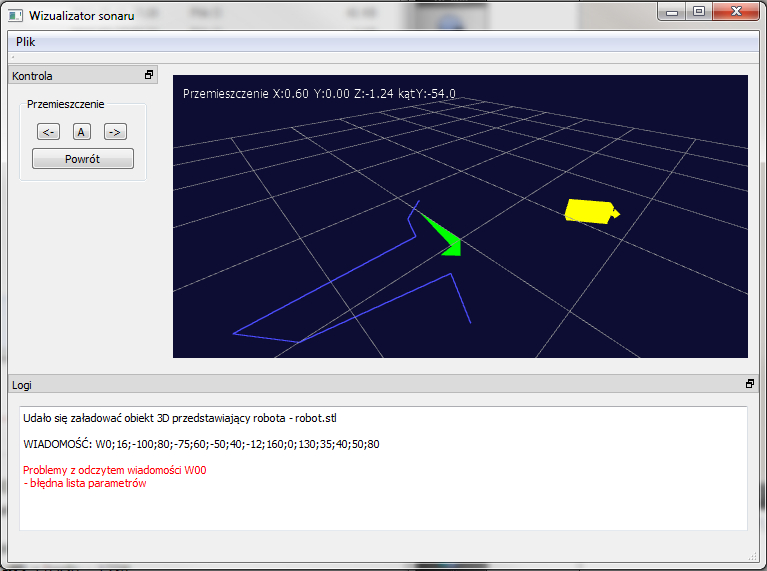
\includegraphics[width=\textwidth]{screen.jpg}
\end{figure}

Poważniejsze błędy, wymagające uwagi użytkownika są raportowane okienkiem błędu. 
\begin{figure} [H]
\centering
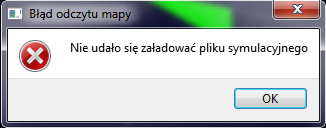
\includegraphics{error_screen.png}
\end{figure}





\section{Diagramy}
Poniżej zaprezentowany został diagram klas dla głównej aplikacji komputerowej. 
Analizę należy rozpocząć od klasy MainWindow, która odpowiada głównemu oknu aplikacji. Przechowuje ona obiekty pozostałych klas. 
MessageController odpowiada za interpretowanie i przygotowywanie wiadomości potrzebnych do komunikacji z urządzeniami oraz odczytem danych z plików.
Będzie ona dziedziczona przez klasy FileController (obsługuje operacje plikowe) oraz RobotController (zarządza robotem). 
W przypadku tej drugiej klasy odziedziczy ona również po klasie BluetoothController. Zapewni to klasie RobotController komplet funkcji potrzebnych
do sterowania robotem. 
Klasa MapViewer dziedziczy od klasy QOpenGLWidget oraz QOpenGLFunctions i odpowiada za sterowanie widokiem 3D.
Klasa EnvMap przechowuje komplet informacji związany z danymi skanowania. Przechowuje ona ją w postaci zbioru wierzchołków przestrzennych, które mogą zostać przekazane do kontekstu OpenGL, oraz dodatkowych zmiennych przechowujących informacje związane ze skalą obiektu, koloru materiału, punktu centralnego czy kątu obrotu.
\newline
W ramach projektu pozostało zaimplementowanie klas BluetoothController oraz częściowo już stworzonej klasy RobotController.

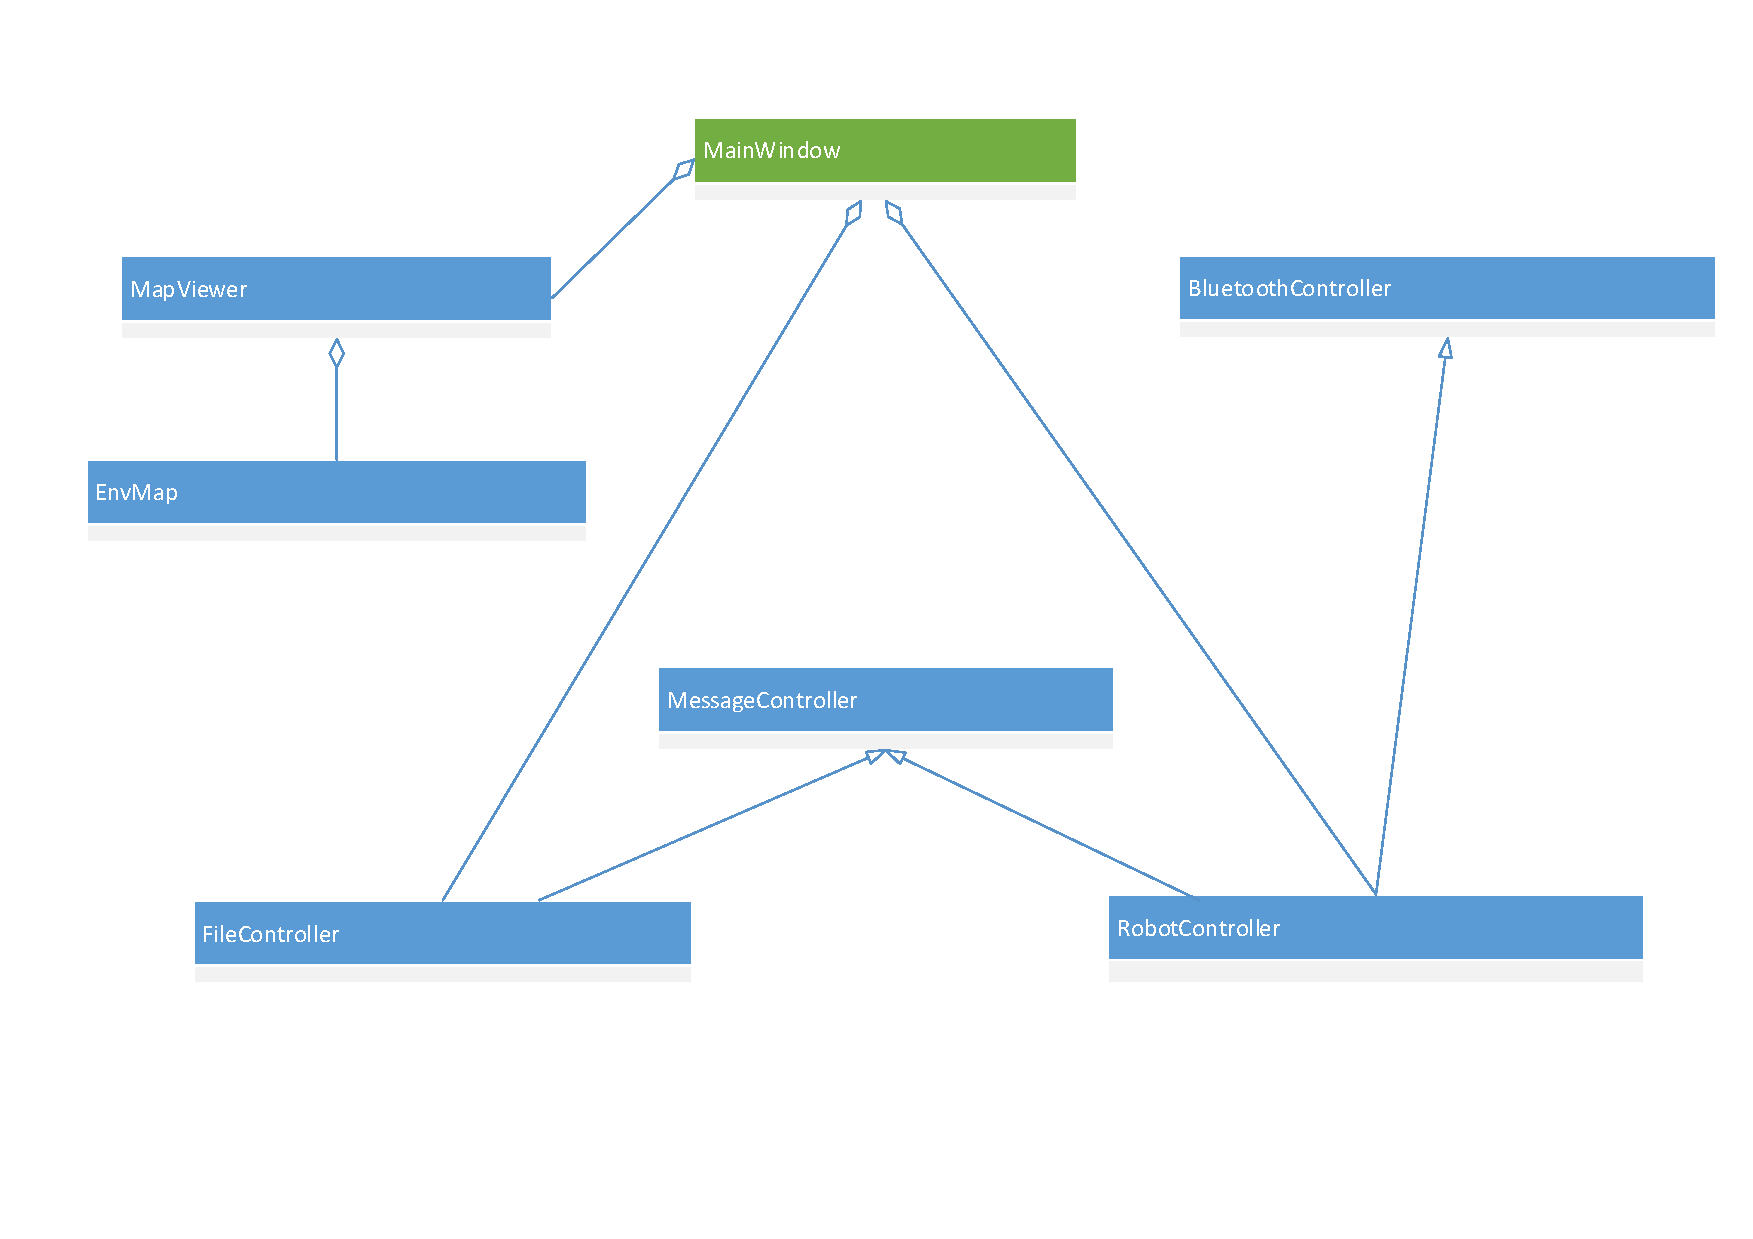
\includepdf[pages={1},landscape=true]{d_klas3.pdf}

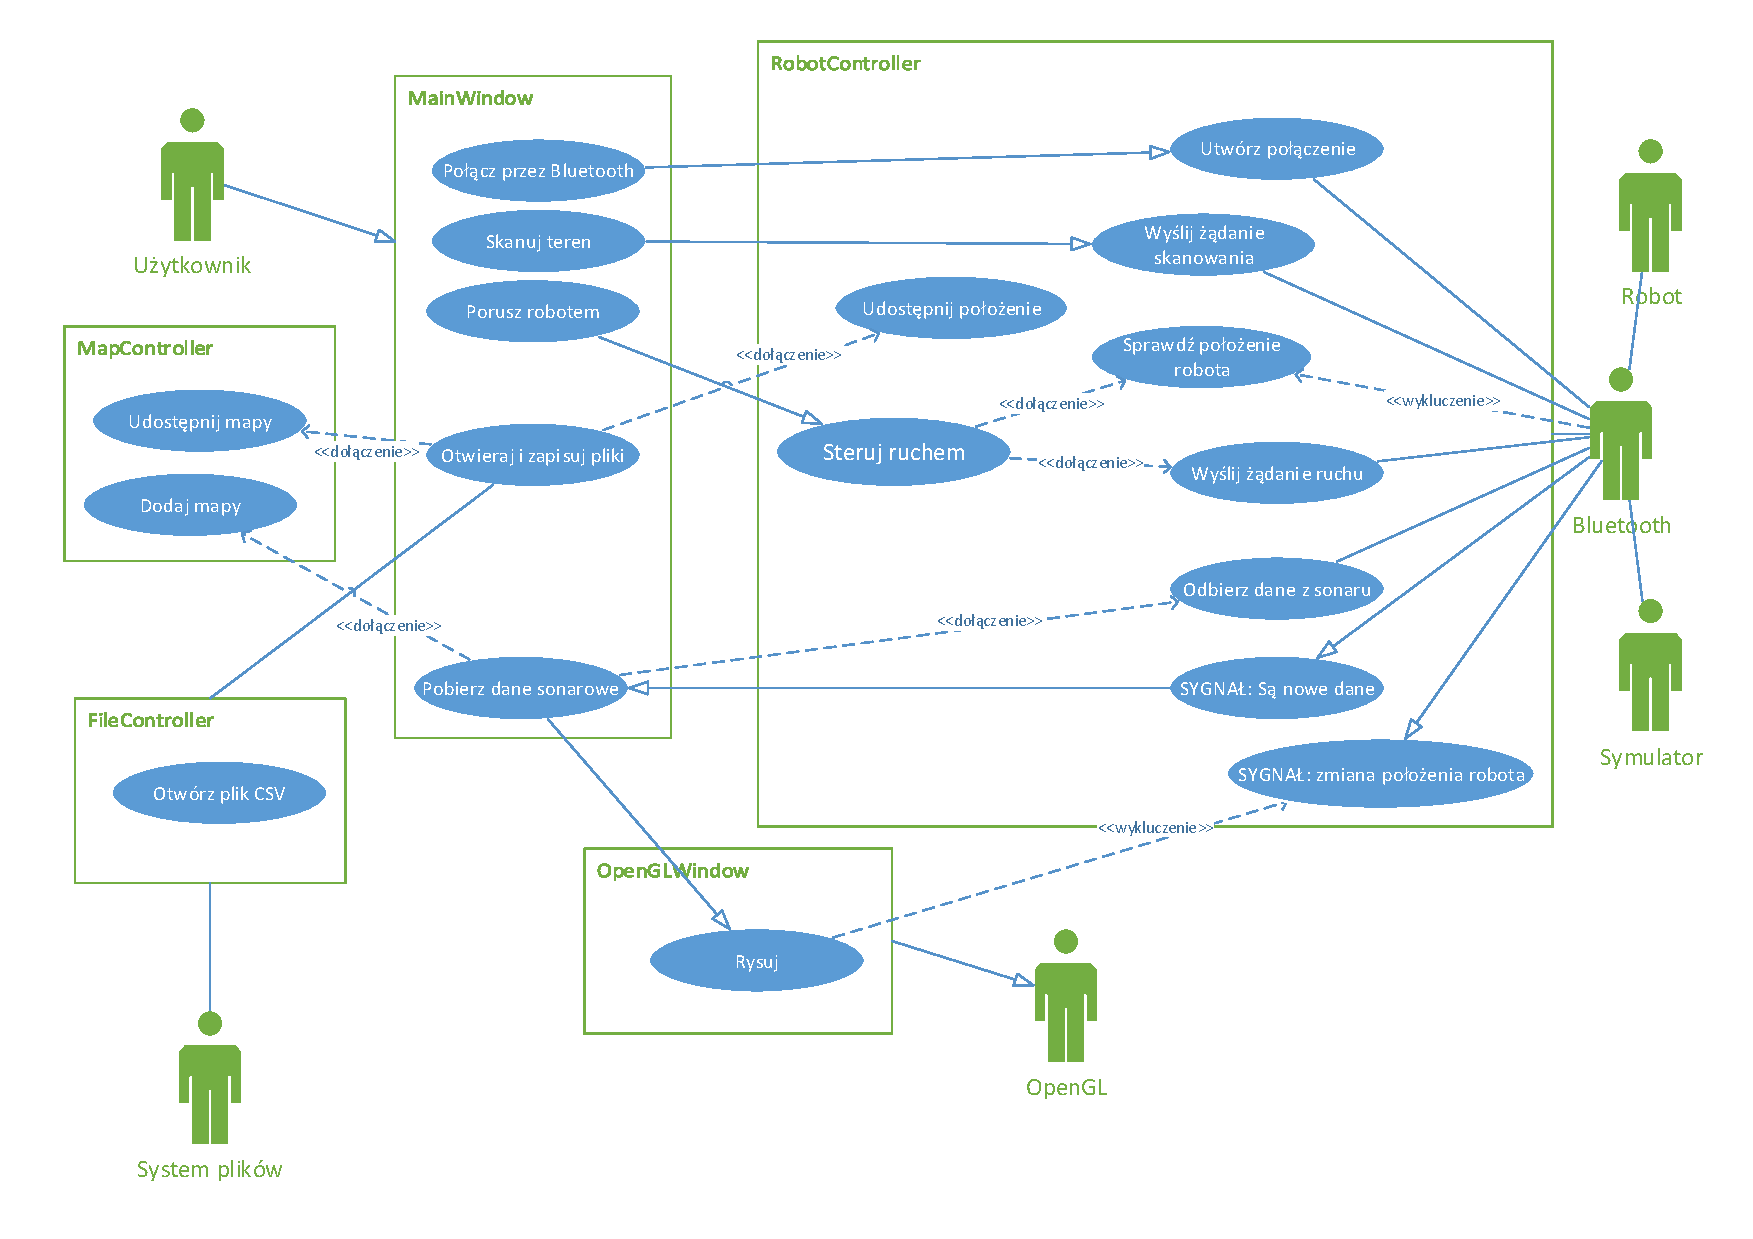
\includepdf[pages={1},landscape=true]{przypadki2.pdf}

\end{document}
